\begin{tcolorbox}[colbacktitle=gray, title={\fontsize{35pt}{0pt}\selectfont 非線形グラフ分類回帰モデル}]
	\structure{回帰木} \\
	\vspace*{-10pt} 
	\vspace{-30pt} \\
\hspace*{770pt}\includegraphics[width=300pt]{img/dtr_drawio.png}
\begin{textblock*}{\textwidth}(000pt,-430pt)
	\vspace*{160pt}
	入力データに対して \\
	内部ノードで質問し最適な分割を行う \\
	葉ノードで定数値を返す \\

	\vspace*{20pt}
	質問 : \\
	ある部分グラフを含むor含まない \\

	\vspace*{20pt}
	勾配ブースティングは分類木ではなく回帰木が必要 
\end{textblock*}
\begin{textblock*}{\textwidth}(925pt,-205pt)
	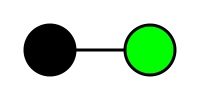
\includegraphics[width=60pt]{img/subgraph/kg.png}
\end{textblock*}
\begin{textblock*}{\textwidth}(820pt,-205pt)
	\scriptsize
	\fontsize{18pt}{0pt} \selectfont含む
\end{textblock*}
\begin{textblock*}{\textwidth}(1040pt,-205pt)
	\scriptsize
	\fontsize{18pt}{0pt} \selectfont含まない
	\end{textblock*}
\begin{textblock*}{\textwidth}(855pt,-100pt)
	\includegraphics[width=60pt]{img/subgraph/wy.png}
\end{textblock*}
\begin{textblock*}{\textwidth}(750pt,-95pt)
	\scriptsize
	\fontsize{18pt}{0pt} \selectfont含む
\end{textblock*}
\begin{textblock*}{\textwidth}(980pt,-95pt)
	\scriptsize
	\fontsize{18pt}{0pt} \selectfont含まない
\end{textblock*}


	\vspace*{-20pt} 
	\structure{勾配ブースティング} \\
	\vspace*{5pt} \\
	加法的アンサンブルモデル
	\begin{equation}
		F(G) = T_0(G) + s T_1(G) + s T_2(G) + s T_3(G) + \cdots
	\end{equation}
	%\vspace{-30pt} \\
	$T_k$ : 各反復における残差$r_i$に対する回帰木.
	\begin{equation}
		r_i = \frac{\partial \mathrm{L}(y_i, F_{k-1}(G_i))}{\partial F}
	\end{equation}
	\color{ash}
	$s$ : 学習率, \hspace{10pt} $\mathrm{L}$ : 損失関数.
	\vspace*{20pt} 

	\color{black}
	\structure{内部ノードにおける分割ルールの学習} \\
	\vspace*{5pt} \\
	二乗誤差和を最小化する分割ルール(部分グラフ)の学習
	\begin{equation}
		\arg\mymin{x_j \in X} \big[ \TSS(D_1(x_j)) + \TSS(D_0(x_j)) \big]
		\label{min:internal}
		\vspace{-5pt}
	\end{equation}
	$X$ : 全部分グラフ集合(\alert{全列挙は困難}) \\
	$D_1(x_j)$ : $ \{x_j$を含むグラフ集合$\}$, \hspace{30pt} $D_0(x_j)$ : $ \{x_j$を含まないグラフ集合$\}$ \\
	$\TSS(D)$ : 残差$r_i$に対する二乗誤差和 \\
	\vspace{-10pt}
\end{tcolorbox}
